%!TEX TS-program = pdflatex
\documentclass[
%draft,
10pt,
%pantone312, 	% WWU-Design in hellblau
%pantone396, 	% WWU-Design in grellem hellgrün 
pantone315, 	% WWU-Design in dunkelblau
%pantone3282, 	% WWU-Design in "blau"
%pantone390, 	% WWU-Design in 
%pantone369,	% WWU-Design in gras-grün
%pantoneblack7, % WWU-Design in dunklem gras-grün
%blackberry,
%handout		% aktivieren um \pause für Druck zu ignorieren (keine neue Seite für einen neuen Punkt)
]{beamer}

\usepackage{longtable}
\usepackage{wwustyle2}
\usepackage[ngerman]{babel}
\usepackage[utf8]{inputenc}
\usepackage[T1]{fontenc}%
\usepackage{multirow}
\usepackage{mathtools}
\usepackage{amsmath}
\usepackage{tabularx}
\usepackage{listings}
\usepackage{textcomp}
\usepackage{tikz-cd}
\usepackage{tikz}
\usetikzlibrary{quotes,babel,arrows,automata,positioning,trees,graphs,shapes,calc,decorations.pathreplacing}
\usepackage{multicol}
\usepackage[]{todonotes}
\usepackage{pgfpages}
\usepackage[%
backend=biber,
sortlocale=auto,
natbib,
hyperref,
backref,
style=alphabetic % eine unvollständige Auswahl von Styles: ieee, numeric, apa
]%
{biblatex}
\addbibresource{quellen.bib} % Literaturdatei einlesen
\setbeamertemplate{bibliography item}[text]


\newcommand{\bet}[1]{\textbf{\textcolor{maincolor}{#1}}}

\lstset{frame=tb,
	language=Java,
	aboveskip=3mm,
	belowskip=3mm,
	showstringspaces=false,
	columns=flexible,
	basicstyle={\small\ttfamily},
	numbers=left,
	frame=single,
	numberstyle=\tiny\color{gray},
	keywordstyle=\bfseries\color{maincolor!60!black},
	commentstyle=\itshape\color{orange!75!black},
	identifierstyle=\color{maincolor!20!black},
	stringstyle=\color{orange!98!black},
	backgroundcolor=\color{gray!10},	
	breaklines=true,
	breakatwhitespace=true,
	tabsize=3
}
\lstset{literate=%
	{Ö}{{\"O}}1
	{Ä}{{\"A}}1
	{Ü}{{\"U}}1
	{ß}{{\ss}}2
	{ü}{{\"u}}1
	{ä}{{\"a}}1
	{ö}{{\"o}}1
}

\newcommand{\java}[1]{\colorbox{gray!20}{\lstinline!#1!}}

\begin{document}
\date{\today}
\author{Jonas Kremer}
\title{Operator Präzedenz Sprachen}
\subtitle{und ihre Automaten}

\setbeamertemplate{section in toc}[sections numbered]
\setbeamertemplate{subsection in toc}[subsections numbered]

\AtBeginSection[]
{
	\begin{frame}[t]
\tableofcontents[currentsection, hidesubsections, hideothersubsections,
	sectionstyle=show/shaded]
	\end{frame}
}

\begin{frame}[plain]
  \maketitle
\end{frame}

\begin{frame}[t]{Agenda}
	\tableofcontents[hidesubsections, hideothersubsections]
\end{frame}

\section{Einleitung}
\begin{frame}[t]{\secname}
	\begin{enumerate}[<+->]
		\item
		Operator Precedence Languages (OPL) sind eine Subklasse der kontextfreien Sprachen
		\item
		Sie wurden 1963 von Robert W. Floyd vorgestellt
		\item
		Größte bekannte Klasse von kontextfreien Sprache, die Abschlusseigenschaften von regulären Sprachen hat
		
	\end{enumerate}	
\end{frame}
\begin{frame}[t]{Motivation}
	\begin{enumerate}[<+->]
		\item 
		Als Beispiel dient eine einfache Sprache für arithmetische Ausdrücke\\
		zB. $ n + n \times (n + n)$
		\item 
		Präzedenz der Multiplikation über die Addition
		\item 
		Parsing basiert auf Operator Präzedenz Relationen, wodurch lokales Parsing und erhöhte Parallelisierung möglich ist
	\end{enumerate}	
\end{frame}

\section{Vorbereitung}
\begin{frame}[t]{Definition kontextfreie Grammatik}
	\begin{itemize}[<+->]
		\item
		Eine kontextfreie Grammatik ist ein 4-Tupel $G = (N, \Sigma , P, S)$
		\begin{enumerate}
			\item
			N ist die Menge der Nichtterminale
			\item
			$\Sigma$ ist die Menge der Terminalsymbole
			\item
			P sind die Produktionsregeln
			\item
			S $\in$ N ist das Startsymbol
		\end{enumerate}
		\item
		Produktionen haben die Form $A \rightarrow \beta$, wobei $\beta \in (\Sigma \cup N) \cup \epsilon$
		\item
		Ableitungen werden mit $\Rightarrow$ bzw. $\xRightarrow{\text{*}}$ beschrieben
		\item
		Definitionen und Namenskonventionen
	\end{itemize}
\end{frame}

\begin{frame}[t]{Namenskonventionen 1}
	\begin{enumerate}
		\item
		$a,b,\dots\in\Sigma$ sind einzelne Terminalsymbole
		\item 
		$u,v, \dots\in\Sigma\textsuperscript{*}$ sind beliebige Terminalstrings
		\item
		$A,B,\dots\in N$ sind einzelne Nichtterminale
		\item
		$\alpha,\beta,\dots\in (\Sigma \cup N)\textsuperscript{*}$ sind beliebige Reststrings
		\item
		$A \rightarrow \epsilon $ ist die \textit{leere Regel}
		\item
		Eine \textit{umbenennende} Regel hat nur ein Nichtterminal als rechte Seite $\left( A \rightarrow B \right)$

	\end{enumerate}
\end{frame}

\begin{frame}[t]{Namenskonventionen 2}
	\begin{itemize}[<+->]
			\item
		Eine Grammatik ist \textit{reduziert}, wenn jede Regel benutzt werden kann um ein Wort aus $\Sigma \textsuperscript{*}$ zu erzeugen
		\item
		Eine. Grammatik ist \textit{invertierbar}, wenn es keine identischen rechten Seiten von Produktionsregeln gibt
		\item
		Eine Regel ist in \textit{Operatorform}, wenn die rechte Seite keine benachbarten Nichtterminale hat
		\item 
		Jede kontextfreie Grammatik kann in eine äquivalente \textit{Operatorgrammatik (OG)} umgewandelt werden
		
		
	\end{itemize}
\end{frame}

\begin{frame}[t] {Bsp. Operator Grammatik}
	\begin{itemize}[<+->]
	\item
	$N=\{E, T, F \}$\\
	E ist das Startsymbol \\
	$\Sigma = \{+, \times, n, (, ) \}$
	\item 
	Produktionsregeln:\\
	$E \rightarrow E + T | T$ \\
	$T \times F | F$ \\
	$F \rightarrow n | (E)$
	
	\end{itemize}
\end{frame}

\section{Operator Präzedenz Grammatik}
\begin{frame}[t]{\subsecname}
	\begin{itemize}[<+->]
		\item
		Definition: \textit{Linke und Rechte Terminalmenge}\\
		$\mathcal{L} \textsubscript{G} \big( A \big) = \{ a \in \Sigma | 
		A \overset{*}{\Rightarrow}Ba \alpha \} $\\
		$\mathcal{R} \textsubscript{G} \big( A \big) = \{ a \in \Sigma | 
		A \overset{*}{\Rightarrow} \alpha aB \}$
		\item
		Es werden drei binäre Operator Präzedenz Relationen definiert:
		\item
		equal in precedence: $ a \doteq b \Leftrightarrow \exists A \rightarrow \alpha aBb \beta , 
		B \in N \cup \{ \epsilon \}$ \\
		takes precedence: $ a \gtrdot b \Leftrightarrow \exists A \rightarrow \alpha Db \beta , D \in N $ and $ a \in
		\mathcal{R}\textsubscript{G}(D)$ \\
		yields precedence: $ a \lessdot b \Leftrightarrow \exists A \rightarrow \alpha aD \beta , D \in N $ and $ b \in
		\mathcal{L}\textsubscript{G}(D)$
		\item Eine Operator Präzedenz Matrix (OPM) M ist eine $|\Sigma| \times |\Sigma |$ Matrix, die für jedes Paar (a,b) die Precedence Relation speichert
		\item 
		Eine Operator Grammatik ist eine Operator Präzedenz Grammatik, wenn M=OPM(G) \textit{konfliktfrei} ist
	\end{itemize}
\end{frame}

\begin{frame}[t] {Beispiel}
	\begin{itemize}[<+->]
	\item
	$\mathcal{L}(E)=\{+, \times, n, (\}, \mathcal{L}(T)=\{\times, n, (\}, \mathcal{L}(F)=\{n,(\}$
	\\
	$\mathcal{R}(E)=\{+, \times, n, )\}, \mathcal{R}(T)=\{\times, n, )\}, \mathcal{R}(F)=\{n,)\}$
	\item
	OPM(G):\\
	\begin{tabular}{c | c c c c c}
	    & + & $\times$ & ( & ) & n \\ \hline
	  + & $\gtrdot$ & $\lessdot$ & $\lessdot$ & $\gtrdot$  &$\lessdot$ \\
	  $\times$ & $\gtrdot$ & $\gtrdot$ & $\lessdot$ & $\gtrdot$ & $\lessdot$ \\
	  ( & $\lessdot$ & $\lessdot$ & $\lessdot$ & $\doteq$ & $\lessdot$\\
	  ) & $\gtrdot$ & $\gtrdot$ &  & $\gtrdot$ & \\
	  n & $\gtrdot$ & $\gtrdot$ &  & $\gtrdot$ & \\
	\end{tabular}
	\\
	\item
	$( \lessdot \times \Leftrightarrow \exists A \rightarrow \alpha (D \beta D \in N $ and $ \times \in
		\mathcal{L}\textsubscript{G}(D)$
	\item
	$ n \gtrdot + \Leftrightarrow \exists A \rightarrow \alpha D+ \beta , D \in N $ and $ n \in
		\mathcal{R}\textsubscript{G}(D)$
	\item
	$ ( \doteq ) \Leftrightarrow \exists A \rightarrow \alpha (B) \beta , 
		B \in N \cup \{ \epsilon \}$
	\end{itemize}
\end{frame}

\begin{frame}[t]{\subsecname}
	\begin{itemize}[<+->]
	\item
	Eine OPG ist in \textit{Fischer Normalform}, wenn sie invertierbar ist und keine leeren (ausser Startsymbol) oder umbenennenden Regeln hat
	\item
	Zusätzliches Symbol $\# \notin \Sigma$ um das Ende eines Strings zu markieren\\
	Alle anderen Symbole übernehmen Precedence über $\#$
	\item
	Ein Operator Präzedenz Alphabet ist ein Paar $(\Sigma, M)$ mit der konfliktfreien OPM $M = | \Sigma \cup \{ \# \} | \textsuperscript{2}$	
	\end{itemize}
\end{frame}



\section{Operator Präzedenz Automaten}
\begin{frame}[t]{\subsecname}
	\begin{itemize}[<+->]
		\item
		Ein nichtdetermistischer Operator Precedence Automat (OPA) ist ein 6-Tupel A = $(\Sigma, M, Q, I, F, \delta)$
		\begin{enumerate}
			\item
			$(\Sigma, M)$ ist ein OP Alphabet
			\item
			Q ist die Menge der Zustände
			\item
			$ I \subseteq Q$ ist die Menge der Startzustände
			\item
			$ F \subseteq Q$ ist die Menge der finalen Zustände
			\item 
			$\delta$ ist die Übergangsfunktion, die aus drei Teilen besteht: \\
			$\delta \textsubscript{shift}: Q \times \Sigma \rightarrow \mathcal{P} (Q)$
			$\delta \textsubscript{push}: Q \times \Sigma \rightarrow \mathcal{P} (Q)$
			$\delta \textsubscript{pop}: Q \times Q \rightarrow \mathcal{P} (Q)$
		\end{enumerate}
		\item
		Weiterhin wird das Stackalphabet definiert als $\Gamma = (\Sigma \times Q)$\\
		mit $\left[a , q \right]\in \Gamma$ und dem Symbol für den leeren Stack ${\perp}$
		\item
		Der Stack $\Pi$ ist ein String $\perp \Gamma \textsuperscript{*}$ \\
		Bsp: $\perp \left[+, q \textsubscript{1} \right] \left[ n, q \textsubscript{0} \right]$
	\end{itemize}
\end{frame}

\begin{frame}[t]{\subsecname}
	\begin{itemize}[<+->]
		\item
1		Eine \textit{Konfiguration} eines OPA ist ein Tripel $C = (\Pi, q, w)$ mit dem Stack $\Pi$, dem aktuellen Zustand q und der Eingabe w
		\item Eine Berechnung des Automaten ist eine endliche Folge von \textit{Transitionen (Moves)} $C \textsubscript{1} \vdash C \textsubscript{2}$
		\item
		Die Sprache die ein OPA A akzeptiert wird definiert als: \\
		L(A)= $\left\{x|(\perp, q \textsubscript{I}, x\#) \vdash \textsuperscript{*} ( \perp, q \textsubscript{F}, \#) ,
		q \textsubscript{I} \in I, q \textsubscript{F} \in F \right\}$
	\end{itemize}
\end{frame}

\begin{frame}[t]{OPA Transitionen}
	\begin{itemize}[<+->]
		\item
		\textit{push move:} (Normaler Pfeil) \\
		if $sym(\Pi) \lessdot a$ then $(\Pi, p, ax) \vdash (\Pi\left[a, p \right], q, x)$ mit 
		$q \in \delta \textsubscript{push} (p,a)$
		\item
		\textit{shift move: } (Gestrichelter Pfeil) \\
		if $a \doteq b$ then $(\Pi\left[a, p \right], q, bx) \vdash (\Pi \left[ b, p \right], r, x)$ mit 
		$r \in \delta \textsubscript{shift} (q, b)$
		\item
		\textit{pop move: } (Doppelter Pfeil) \\
		if $ a \gtrdot b$ then $(\Pi\left[a, p\right], q, bx) \vdash (\Pi, r, bx)$ mit $r \in \delta \textsubscript{pop} (q,p)$
	
	\end{itemize}
\end{frame}

\subsection*{Automaten Beispiel}
\begin{frame}[t]{\secname}
	\begin{figure}
	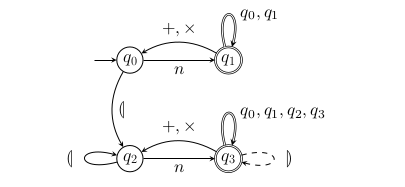
\includegraphics[width=10cm,height=5cm]{img/opa.png}
	\end{figure}
\end{frame}
\begin{frame}
	\small
	\begin{tabular}{| l | c | r |}
	\hline
	Stack & Zustand & Eingabe \\ \hline
	$\perp$ & $q \textsubscript{0}$ & $ n+n \times (n+n)\#$ \\ \hline
	
	$ \perp\left[n, q\textsubscript{0} \right]$ & $q \textsubscript{1}$ & $+n \times (n+n)\#$ \\ \hline
	
	$\perp$ & $q \textsubscript{1}$ & $ +n \times (n+n)\#$ \\ \hline
	
	$\perp\left[+, q\textsubscript{1} \right]$ & $q \textsubscript{0}$ & $ n \times (n+n)\#$ \\ \hline
	
	$\perp\left[+, q\textsubscript{1} \right] \left[n, q\textsubscript{0} \right]$ 
	& $q \textsubscript{1}$ & $\times (n+n)\#$ \\ \hline
	
	$\perp\left[+, q\textsubscript{1} \right]$ & $q \textsubscript{1}$ & $\times (n+n)\#$ \\ \hline
	
	$\perp\left[+, q\textsubscript{0} \right]\left[\times, q\textsubscript{1} \right]$ 
	& $q \textsubscript{1}$ & $(n+n)\#$ \\ \hline
	
	$\perp\left[+, q\textsubscript{1} \right]\left[\times, q\textsubscript{1} \right] \left[(, q\textsubscript{0} \right]$ 
	& $q \textsubscript{2}$ & $n+n)\#$ \\ \hline
	
	$\perp\left[+, q\textsubscript{1} \right]\left[\times, q\textsubscript{1} \right] \left[(, q\textsubscript{0} \right] \left[n, q\textsubscript{2} \right]$ 
	& $q \textsubscript{3}$ & $+n)\#$ \\ \hline
	
	$\perp\left[+, q\textsubscript{1} \right]\left[\times, q\textsubscript{1} \right] \left[(, q\textsubscript{0} \right]$ 
	& $q \textsubscript{3}$ & $+n)\#$ \\ \hline
	
	$\perp\left[+, q\textsubscript{1} \right]\left[\times, q\textsubscript{1} \right] \left[(, q\textsubscript{0} \right] \left[+, q\textsubscript{3} \right]$ 
	& $q \textsubscript{2}$ & $n)\#$ \\ \hline
	
	$\perp\left[+, q\textsubscript{1} \right]\left[\times, q\textsubscript{1} \right] \left[(, q\textsubscript{0} \right] \left[+, q\textsubscript{3} \right] \left[n, q\textsubscript{2} \right]$ 
	& $q \textsubscript{3}$ & $)\#$ \\ \hline
	
	$\perp\left[+, q\textsubscript{1} \right]\left[\times, q\textsubscript{1} \right] \left[(, q\textsubscript{0} \right] \left[+, q\textsubscript{3} \right]$ 
	& $q \textsubscript{3}$ & $)\#$ \\ \hline
	
	$\perp\left[+, q\textsubscript{1} \right]\left[\times, q\textsubscript{1} \right] \left[(, q\textsubscript{0} \right]$ 
	& $q \textsubscript{3}$ & $)\#$ \\ \hline
	
	$\perp\left[+, q\textsubscript{1} \right]\left[\times, q\textsubscript{1} \right] \left[), q\textsubscript{0} \right]$ 
	& $q \textsubscript{3}$ & $\#$ \\ \hline
	
	$\perp\left[+, q\textsubscript{1} \right]\left[\times, q\textsubscript{1} \right]$ 
	& $q \textsubscript{3}$ & $\#$ \\ \hline
	
	$\perp\left[+, q\textsubscript{1} \right]$ 
	& $q \textsubscript{3}$ & $\#$ \\ \hline
	
	$\perp$ 
	& $q \textsubscript{3}$ & $\#$ \\ \hline
	\end{tabular}
	
\end{frame}


\section{(Abschluss-) Eigenschaften von OPLs}
\begin{frame}[t]{OPG $\rightarrow$ OPA}
	\begin{itemize}[<+->]
	\item
	Zu jeder OPG G kann ein OPA A konstruiert werden, sodass gilt L(G)=L(A)
	\item
	Idee: \\
	Man konstruiert einen Automaten, sodass eine erfolgreiche Berechnung \glqq bottom-up \grqq einen Ableitungsbaum erzeugt
	\item
	 Eine Push-Transition wird hinzugefügt, wenn das erste Terminal einer neuen rechten Seite einer Regel gelesen wird. \\
	Ein Shift Move bei Terminalen innerhalb einer Regel.\\
	Ein Pop Move am Ende einer rechten Seite.
	\item
	Jeder Zustand enthält das Präfix der rechten Seite einer Regel die gerade konstruiert wird und Informationen zu dem Zustand der vorher konstruiert wurde
	\item
	Sei m die Summe der Längen der rechten Seiten einer Regel. \\
	Dann hat A O($m \textsuperscript{2}$) Zustände
	
	\end{itemize}
\end{frame}

\begin{frame}[t]{OPA $\rightarrow$ OPG}
	\begin{itemize}[<+->]
	\item
	Zu jedem OPA A kann eine OPG G konstruiert werden, sodass gilt L(A)=L(G)
	\item
	Die Nichtterminale haben die Form $\Sigma \times Q \times Q \times \Sigma$
	\item
	Idee: \\
	Man definiert sogenannte Supports (Transitionspfade) für einfache und zusammengesetzte Ketten von Terminalen
	\item
	Eine einfache Kette ist ein String von Nichtterminalen sodass gilt: $a \textsubscript{0} \lessdot a \textsubscript{1} \doteq a \textsubscript{2} \doteq ... \doteq a \textsubscript{n} \gtrdot a \textsubscript{n+1}$ \\
	Schreibweise:  $\textsuperscript{a \textsubscript{0}}( a \textsubscript{1},..., a \textsubscript{n}) \textsuperscript{a \textsubscript{n+1}}$
	\item
	Bei zusammengesetzten Ketten werden zwischen den einzelnen Terminalen einer einfachen Kette eine weitere Kette eingefügt
	\item
	Für jeden Support wird in einer bestimmten Weise eine Regel erzeugt 
	
	\end{itemize}
\end{frame}

\begin{frame}[t]{\secname}
	\begin{itemize}[<+->]
	\item 
	OPLs sind eine große Subklasse der kontextfreien Sprachen\\
	$L=\{ a \textsuperscript{n} b a \textsuperscript{n} | n \geq 0\}$ kann nicht durch OPG dargestellt werden
	\item
	Abgeschlossen unter Vereinigung, Schnitt, Komplement, Konkatenation und Kleene-*
	\item
	Das Leereproblem ist in PTIME lösbar, da OPLs Subklasse von kfG	
	\end{itemize}
\end{frame}


\begin{frame}[t]{Deterministischer vs Nichtdeterministischer OPA}
	\begin{itemize}
	\item
	Ein OPA ist deterministisch, wenn $|I| = 1$ und $\delta \textsubscript{push}, \delta \textsubscript{shift}, \delta \textsubscript{pop}$ auf Q anstatt $\mathcal{P}(Q)$ abbilden
	\item
	Zu jedem nichtdeterministischen OPA mit s Zuständen kann ein äquivalenter deterministischer OPA mit $2 \textsuperscript{O(s \textsuperscript{2})}$ Zuständen erzeugt werden
	\end{itemize}
\end{frame}


\section{Ausblick}
\begin{frame}[t]{\secname}
	\begin{itemize}[<+->]
	\item
	Visibly Pushdown Sprachen als Subklasse von OPL
	\item
	Monadic Second Order Logic Characterization
	\item
	$\omega$-Operator Präzedenz Sprachen
	\item
	Implementierung eines Operator Präzedenz Automaten
	\end{itemize}
\end{frame}

\nocite{*}
\section*{Quellen}
\begin{frame}{Quellen}
\begin{thebibliography}{9}
\bibitem{unimilano} 
Violetta Lonati, Dino Mandrioli, Matteo Pradella
\textit{Precedence Automata and Languages}. 
Milano, Italy
\bibitem{siam}  
Violetta Lonati, Dino Mandrioli, Matteo Pradella, Frederica Panella
\textit{Operator Precedence Languages: their automata-theoretic and logic characterization} 
[\textit{SIAM J. Comput. 2015 Society for Industrial and Applied Mathematics}]. 

 
\bibitem{property} 
Stefano Crespi Reghizzi, Dino Mandrioli
\textit{Operator precedence and the visibly pushdown property}
[\textit{Journal  of Computer and System Sciences}].
\end{thebibliography}
\end{frame}

\end{document}
